\section{Analisis Solusi}

\subsection{Ide Dasar}

Berikut adalah ide dasar untuk menyelesaikan masalah pembacaan ketersediaan tiket dan pemesanan tiket:

\begin{enumerate}
  \item Tanggung jawab pelayanan ketersediaan tiket dapat dilimpahkan kepada RisingWave, sehingga beban pada basis data berkurang. \textit{Streaming database} ini dapat memperbarui hasil kueri secara inkremental setiap kali ada perubahan. Pendekatan ini mengurangi proses agregasi yang dilakukan secara berulang-ulang, sehingga kueri lebih efisien. Pendekatan ini merupakan bagian dari \textit{query responsibility segregation} pada pola CQRS.
  \item Menggunakan kluster PostgreSQL dengan ekstensi Citus dan pembagian data berdasarkan baris. Pendekatan ini meungkinkan adanya \textit{multiple writer}, sehingga \textit{throughput} pemesanan tiket dapat meningkat. Di sisi lain, tidak menggunakan basis data relasional juga bisa menjadi opsi. Pendekatan \textit{database inside-out} yang memisahkan komponen \textit{storage} dan \textit{query} memungkinkan setiap komponen \textit{scale} secara independen. Meskipun begitu, perlu perhatian khusus untuk menghindari pemesanan ganda dan menjaga integritas transaksi.
  \item Untuk mengontrol pemesanan tiket, pendekatan penyeimbangan beban berbasiskan antrean dapat digunakan. Pemesanan tiket dapat didesain sebagai \textit{command} pada pola CQRS. Dengan begini, sistem dapat memproses permintaan sesuai dengan kapasitas sistem, sehingga stabilitas sistem dapat terjaga. Selain itu, informasi tiket yang sedang dipesan tetapi belum \textit{commit} (kita sebut \textit{uncommited data}) dapat disimpan pada Redis yang kemudian digunakan untuk menolak permintaan lebih awal dan mengurani permintaan yang masuk.
\end{enumerate}

\subsection{Komponen Sistem Tiket}

Berdasarkan studi yang sudah dibahas sebelumnya dan berdasarkan fokus yang ingin dibahas pada penelitian ini, berikut adalah komponen sistem yang menjadi bahasan dari penelitian ini:

\begin{enumerate}
  \item Layanan \textit{backend} utama yang memproses setiap permintaan yang berkaitan dengan pemesanan tiket.
  \item Layanan otentikasi.
  \item Layanan gerbang pembayaran. Layanan ini merupakan layanan eksternal dan cukup melakukan \textit{mocking service}.
  \item Terdapat satu basis data utama sebagai sumber kebenaran utama.
\end{enumerate}

Daftar acara dan ketersediaan awal tiket merupakan data yang diisi dari awal, sehingga fitur manajemen acara dan tiket tidak diimplementasikan. Detail lengkap komponen dan fitur sistem dijelaskan pada bagian lampiran.

\subsection{Arsitektur Solusi}

Komponen \textit{backend} utama bersifat \textit{stateless}, sehingga dapat di-\textit{scale} dengan meningkatkan jumlah \textit{instance}. Setiap arsitektur solusi memiliki dua layanan eksternal, yaitu layanan pengguna dan layanan gerbang pembayaran. Basis data merupakan komponen yang sulit di-\textit{scale} secara dinamis berdasarkan beban yang diterima. Biasanya, penskalaan secara vertikal merupakan opsi utama untuk meningkatkan \textit{throughput}.

\subsubsection{Arsitektur Dasar Acuan}

\begin{figure}[ht]
  \centering
  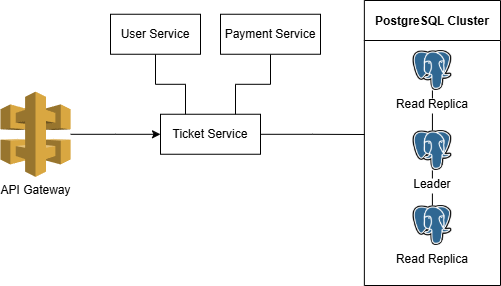
\includegraphics[width=0.8\textwidth]{resources/chapter-3/architecture-reference.png}
  \caption{Arsitektur Dasar Acuan}
  \label{fig:baseline-architecture}
\end{figure}

Arsitektur ini akan menjadi dasar acuan yang digunakan sebagai dasar perbandingan kinerja. Terdapat kluster PostgreSQL dengan konfigurasi satu node pemimpin dan sisanya node replika. Keberadaan replika memungkinkan peningkatan \textit{throughput} permintaan baca, tetapi tidak ada pengoptimalan untuk operasi tulis.

\subsubsection{Arsitektur yang Mengoptimalkan PostgreSQL}

Arsitektur ini mengoptimalkan sistem dengan pola CQRS. Tanggung jawab permintaan baca dilimpahkan kepada RisingWave. \textit{Streaming database} ini mengonsumsi \textit{CDC stream} dari kluster PostgreSQL, lalu memperbarui kueri secara inkremental. Penggunaan ekstensi Citus memungkinkan pembagian data berdasarkan baris dan \textit{multiple writer}. Selain itu, perintah pemesanan tiket (berupa \textit{command}/ \textit{event sourcing}) akan dimasukkan ke dalam antrean terlebih dahulu, lalu diproses secara bertahap. Redis digunakan untuk menyimpan \textit{uncommited data} dan menolak permintaan pemesanan lebih awal.

\begin{figure}[ht]
  \centering
  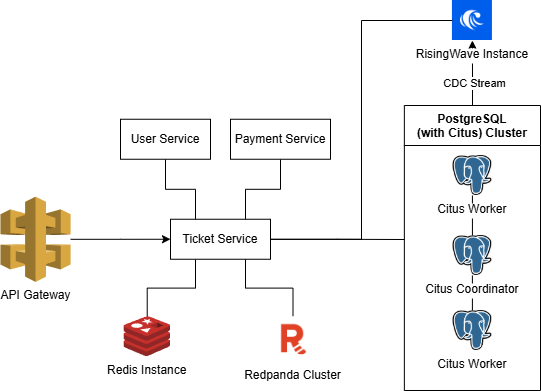
\includegraphics[width=0.8\textwidth]{resources/chapter-3/architecture-optimized.png}
  \caption{Arsitektur yang Mengoptimalkan PostgreSQL}
  \label{fig:optimized-architecture}
\end{figure}

Penggunaan ekstensi Citus memungkinkan penginkatan \textit{write throughput} tidak hanya dengan pendekatan \textit{scale up}, tetapi juga dengan pendekatan \textit{scale-out}. Redpanda dapat dibuat kluster dengan pemartisian data untuk meningkatkan \textit{throughput}. Redis dapat dikonfigurasikan dalam mode kluster untuk redundansi dan mode AOF untuk \textit{persistence}.

\subsubsection{Arsitektur \textit{Event-Driven}}

Arsitektur ini tidak menggunakan PostgreSQL sama sekali. Pada dasarnya, basis data relasional terdiri atas komponen \textit{storage} dan \textit{query processor}. Pada arsitektur ini, komponen \textit{storage} diganti menggunakan Redpanda dengan berbagai topik dan \textit{query processor} diganti dengan RisingWave. Meskipun begitu, pendekatan ini tidak memiliki dukungan \textit{transaction} selain \textit{transaction} pada Redpanda yang berupa \textit{push log all or nothing} pada beberapa topik sekaligus. Untuk itu, Redis digunakan untuk menyimpan \textit{dirty data} atau \textit{uncommited data} sehingga untuk mencegah \textit{double booking}.

\begin{figure}[ht]
  \centering
  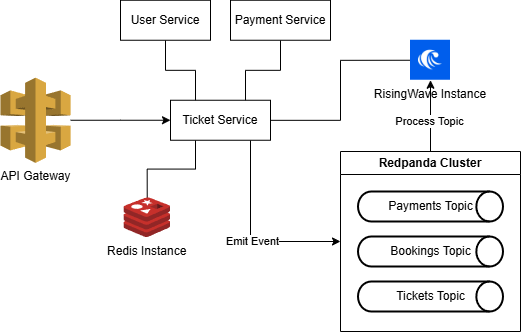
\includegraphics[width=0.8\textwidth]{resources/chapter-3/architecture-event-driven.png}
  \caption{Arsitektur \textit{Event-Driven}}
  \label{fig:solution-event-driven-architecture}
\end{figure}

Redpanda dapat dibuat kluster dengan pemartisian data untuk meningkatkan \textit{throughput}. Redis dapat dikonfigurasikan dalam mode kluster untuk redundansi dan mode AOF untuk \textit{persistence}. Selain itu, RisingWave merupakan \textit{streaming database} yang \textit{cloud-native} sehingga dapat di-\textit{scale out} dengan mudah untuk meningkatkan \textit{throughput}.

% \bgroup
% \begin{table}[ht]
%   \def\arraystretch{1.3}
%   \caption{Perbandingan Ketiga Alternatif Solusi}
%   \label{tab:perbandingan-analisis-solusi}
%   \centering
%   \begin{tabular}{|p{2cm}|p{2cm}|p{2cm}|p{1.8cm}|p{1.7cm}|p{1.7cm}|}
%     \hline
%     Solusi           & Berjalan di berbagai perangkat                            & Melakukan \textit{targeted deployment} & Berjalan pada perangkat dengan sumber daya terbatas & Mengatur banyak perangkat & Waktu pembuatan sistem \\
%     \hline
%     Kubernetes       & Ya, seluruh perangkat yang dapat melakukan kontainerisasi & Ya                                     & Ya dengan K3s                                       & Ya                        & Cepat                  \\
%     \hline
%     Zookeper         & Ya, seluruh perangkat yang memiliki java                  & Tidak                                  & Tidak                                               & Ya                        & Cepat                  \\
%     \hline
%     LEONORE \& DIANE & Tidak                                                     & Tidak                                  & Mungkin                                             & Ya                        & Lama                   \\
%     \hline
%   \end{tabular}
% \end{table}
% \egroup